\documentclass[conference]{IEEEtran}

\usepackage[T2A]{fontenc}
\usepackage[utf8]{inputenc}
\usepackage[english,russian]{babel}
\usepackage{lmodern}
\usepackage{amsmath}
\usepackage{graphicx}
\usepackage{booktabs}
\usepackage{cite}
\usepackage{url}

\title{Сравнительное исследование методов машинного обучения, глубокого обучения и фундаментальных моделей для краткосрочного прогнозирования электрической нагрузки}

\author{
\IEEEauthorblockN{Автор Один}
\IEEEauthorblockA{\textit{Аффилиация Один}\\
Город, Страна\\
email1@example.com}
\and
\IEEEauthorblockN{Автор Два}
\IEEEauthorblockA{\textit{Аффилиация Два}\\
Город, Страна\\
email2@example.com}
}

\begin{document}
\maketitle

\begin{abstract}
Краткосрочное прогнозирование электрической нагрузки является ключевым компонентом эксплуатации интеллектуальных энергосетей, опережающего планирования и промышленного энергоменеджмента. В работе представлен воспроизводимый бенчмарк, сравнивающий два классических базовых метода (SeasonalNaive и грид-настроенный SARIMA), модель градиентного бустинга (XGBoost), три нейросетевые архитектуры (DLinear, PatchTST, iTransformer) и две фундаментальные модели временных рядов (Chronos-Bolt-Small и TimesFM~2.5). Основная оценка проводится на наборе ECL по агрегированной нагрузке. ETTh1 используется как вторичный промышленный бенчмарк с целевой переменной HUFL; температура масла OT целенаправленно не рассматривается как электрическая нагрузка. Эксперименты охватывают горизонты 24, 96 и 168 часов при фиксированном контексте 336 часов. На ECL три лидирующие модели --- TimesFM, Chronos-Bolt и XGBoost --- отличаются друг от друга в пределах примерно $0.1$--$0.4\%$ по горизонтам: TimesFM незначительно лучше при H=24, XGBoost --- при H=96 и H=168; грид-настроенный SARIMA закрывает большую часть оставшегося разрыва без обучаемых признаков. На ETTh1/HUFL Chronos-Bolt лучшая при H=24, DLinear --- при H=96 и H=168. Результаты показывают, что фундаментальные модели конкурентоспособны в zero-shot режиме, но классические и обучаемые на целевом ряду модели остаются сильными при наличии данных и инженерии признаков.
\end{abstract}

\begin{IEEEkeywords}
краткосрочное прогнозирование нагрузки, временные ряды, глубокое обучение, фундаментальные модели, SARIMA, XGBoost, интеллектуальная сеть
\end{IEEEkeywords}

\section{Введение}
Краткосрочное прогнозирование нагрузки (STLF) поддерживает диспетчерское планирование, балансировку, тарифно-ориентированное управление, планирование обслуживания и аномально-чувствительный промышленный энергоменеджмент. В современных задачах smart-grid и Industry 4.0 от моделей прогноза требуется не только точность, но и воспроизводимость, вычислительная экономичность и устойчивость к различным режимам эксплуатации.

Методологический ландшафт широк. Классические методы, такие как ARIMA-семейство и сезонные наивные базовые модели, остаются важными референсами; модели машинного обучения вроде градиентного бустинга привлекательны тем, что включают лаговые и календарные признаки при умеренной инженерии; современные модели глубокого обучения и фундаментальные модели обещают более широкую переносимость между доменами временных рядов. Это порождает практический вопрос: когда дорогие архитектуры или zero-shot фундаментальные модели действительно превосходят сильные недорогие базовые методы?

В работе представлено воспроизводимое исполнение бенчмарка на двух открытых наборах данных. Прагматический вклад: (i) сквозной репозиторий с валидацией данных, leakage-aware шкалированием, метриками, измерением времени, фигурами и сборкой статьи; (ii) реальные результаты для SeasonalNaive, грид-настроенного SARIMA, XGBoost, DLinear, PatchTST, iTransformer, Chronos-Bolt-Small и TimesFM~2.5; (iii) тесты Дибольда--Мариано, рассчитанные по поокно-ошибкам; (iv) анализ accuracy--latency, отделяющий стоимость развёртывания от чистой точности.

\section{Обзор литературы}
Классические методы прогнозирования временных рядов, в частности ARIMA-семейство, остаются важными, потому что задают интерпретируемые и недорогие референсы; автоматический выбор порядков по информационным критериям, таким как AICc, делает их применимыми по отдельным рядам \cite{hyndman2008automatic}. Подходы машинного обучения на основе лагов, календарных переменных и градиентно-бустированных деревьев широко используются в задачах прогнозирования нагрузки благодаря быстрому обучению и устойчивости при инженерии табличных признаков \cite{chen2016xgboost}. Модели глубокого обучения, такие как LSTM \cite{hochreiter1997lstm}, архитектуры с механизмом внимания \cite{vaswani2017attention}, Informer \cite{zhou2021informer}, DLinear \cite{zeng2023dlinear}, PatchTST \cite{nie2023patchtst}, iTransformer \cite{liu2024itransformer}, TimesNet \cite{wu2023timesnet}, существенно расширили инструментарий долгосрочного прогнозирования.

Фундаментальные модели временных рядов, такие как TimesFM~\cite{das2024timesfm} и семейство Chronos~\cite{ansari2024chronos}, мотивируют новую ось оценки: безобучаемое инференс-время против полноценного обучения на целевом наборе. В данной работе используется дистиллированный вариант Chronos-Bolt-Small. Корректное сравнение должно учитывать риск того, что открытые бенчмарки могли быть включены в претрейнинговые корпуса, поэтому zero-shot результаты на ECL или ETT нельзя интерпретировать как гарантированную обобщающую способность на невиданных данных.

\section{Методология}
При заданном одномерном контекстном окне $\mathbf{x}_{t-L+1:t}$ задача --- предсказать $\hat{\mathbf{y}}_{t+1:t+H}$ для горизонтов $H \in \{24,96,168\}$. Эксперименты используют фиксированную длину контекста $L=336$ часов, что включает суточную и недельную сезонные компоненты и допускает использование лага 168.

Базовая модель SeasonalNaive повторяет последний наблюдённый суточный сезонный паттерн. Базовая модель SARIMA использует выбор по AICc на тренировочной выборке из фиксированного грида: пробуются порядки $(p,d,q)\in\{(1,1,1),(2,1,1),(1,1,2),(2,1,2)\}$ и сезонные порядки $(P,D,Q)_{24}\in\{(1,1,1),(2,1,1),(1,1,2)\}$, и далее минимально-AICc-фит применяется к каждому тестовому окну через фильтрацию состояния, без переподгонки на каждом окне. XGBoost обучается как прямой многошаговый регрессор на лагах 1, 24, 168, скользящих средних по 24 и 168 часам и циклических календарных признаках. DLinear, PatchTST и iTransformer обучаются через NeuralForecast в той же одноцелевой постановке, с коротким validation-only перебором learning-rate по $\{10^{-3}, 5\cdot10^{-4}\}$ и ранним остановом. Обучение и оценка нейросетевых моделей используют rolling-origin cross-validation в NeuralForecast: хотя train, validation и test конкатенируются для построения скользящих окон, каждое окно прогнозируется только по прошлым наблюдениям, поэтому утечки будущей информации в обучение нет. Chronos-Bolt-Small и TimesFM~2.5 оцениваются в zero-shot режиме без обучения на целевом ряду. Все процедуры предобработки для обучаемых моделей подгоняются только на тренировочной части, а метрики считаются после обратного преобразования предсказаний на исходную шкалу. Фундаментальные модели и SARIMA оцениваются непосредственно в исходной шкале.

Рис.~\ref{fig:methodology} обобщает экспериментальный пайплайн.

\begin{figure}[t]
  \centering
  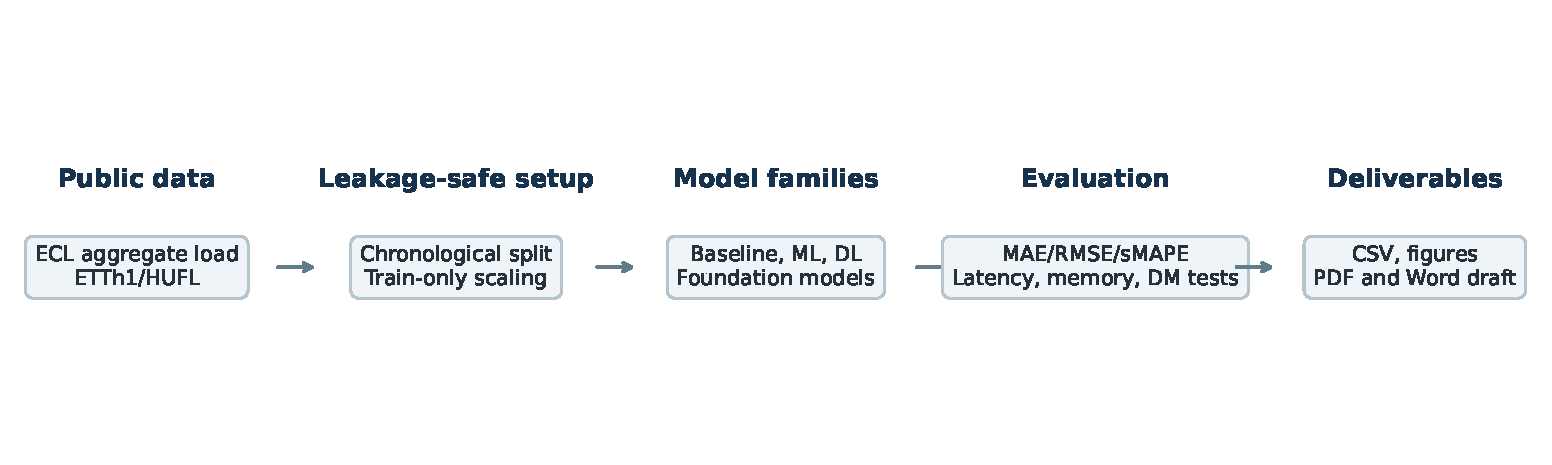
\includegraphics[width=\linewidth]{../figures/fig1_methodology.pdf}
  \caption{Экспериментальный пайплайн.}
  \label{fig:methodology}
\end{figure}

\section{Постановка эксперимента}
Основной набор данных --- ECL, обработанный как агрегированная часовая электрическая нагрузка по 321 клиенту. Вторичный набор --- ETTh1, целевая переменная HUFL. Переменная OT в ETTh1 --- температура масла и не рассматривается как электрическая нагрузка. ECL разбивается хронологически 70\% train, 10\% validation, 20\% test. ETTh1 использует стандартное хронологическое разбиение 12 / 4 / 4 месяца.

Точность измеряется метриками MAE, RMSE, sMAPE и wMAPE. Эффективность измеряется временем обучения, single-window inference latency (batch size~1), числом обучаемых параметров и пиковым потреблением GPU-памяти. Обучаемые модели (XGBoost, DLinear, PatchTST, iTransformer) оцениваются по пяти сидам (42--46) и приводятся как среднее~$\pm$~СКО; детерминированные модели (SeasonalNaive, SARIMA, Chronos-Bolt, TimesFM) оцениваются однократно и имеют нулевое стандартное отклонение по построению. Тесты Дибольда--Мариано вычисляются по поокно-ошибкам для двух топ-моделей по MAE при сиде 42 для каждой пары (датасет, горизонт). Поскольку усреднение по окнам и плоский поточечный MAE взвешивают ошибки по-разному, ранжирование по статистическим тестам может слегка отличаться от ранжирования таблиц при близких моделях.

\section{Результаты}
\begin{figure}[t]
  \centering
  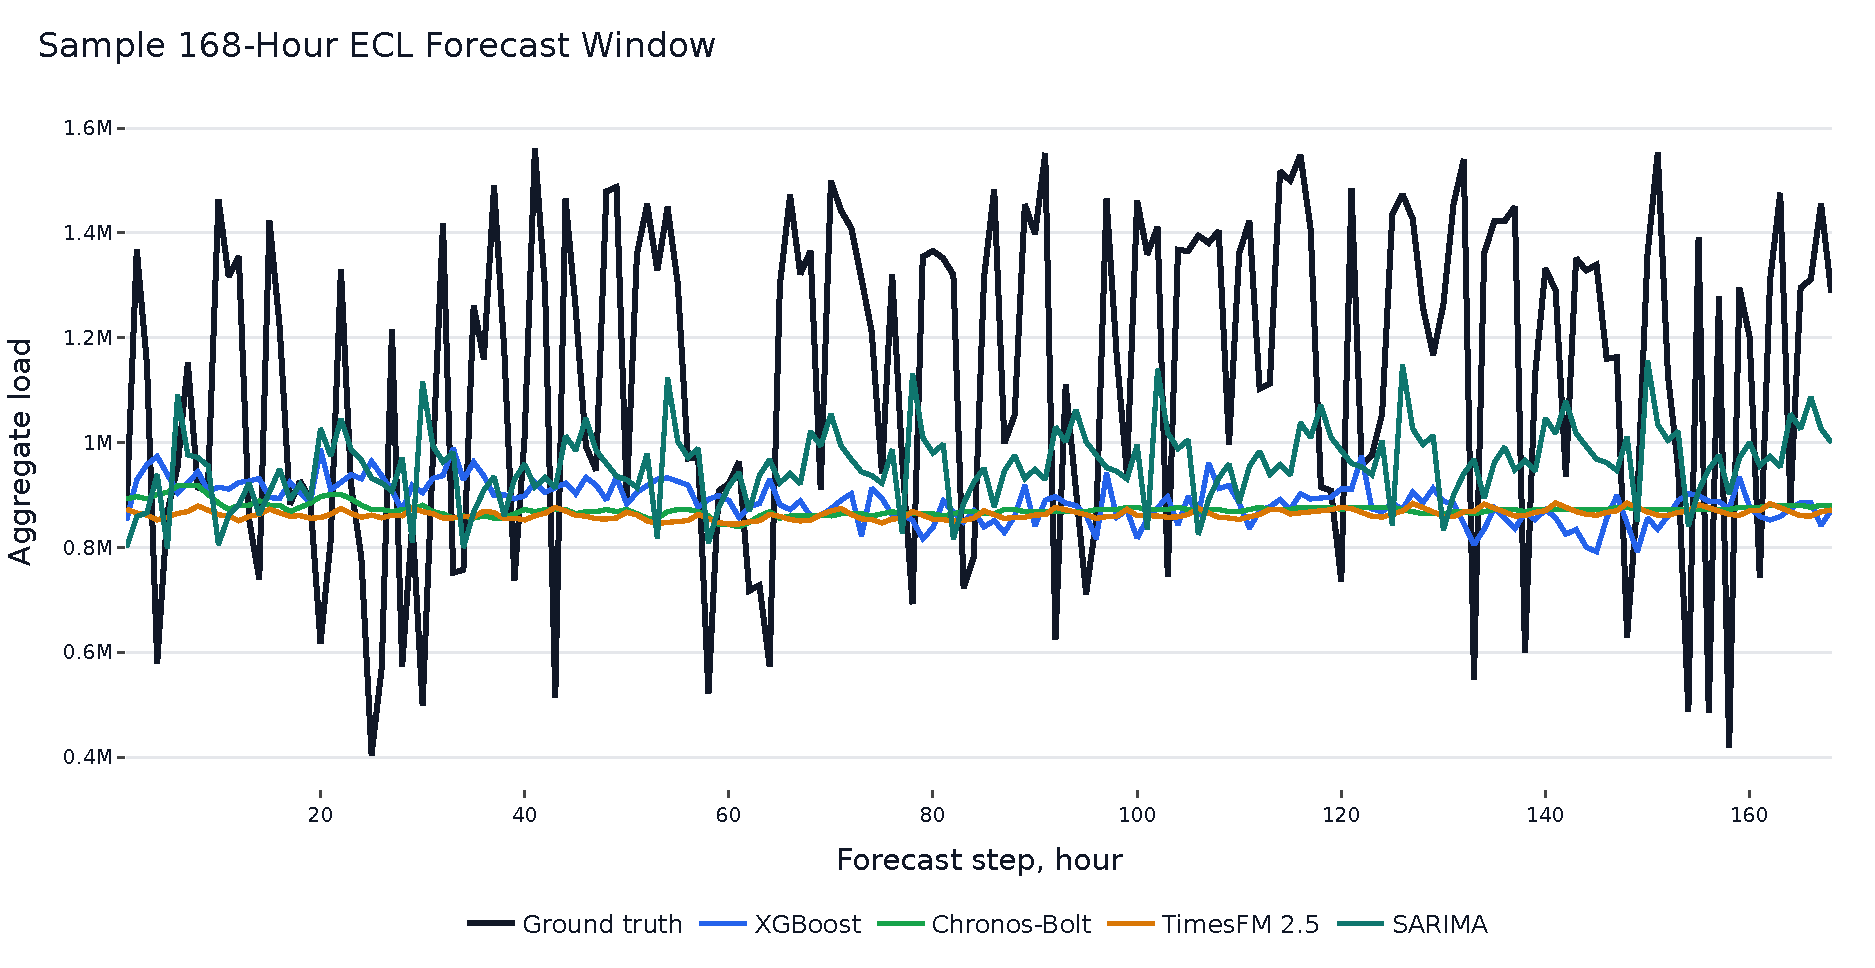
\includegraphics[width=\linewidth]{../figures/fig2_forecasts.pdf}
  \caption{Пример прогнозов на 168 часов для ECL у репрезентативных моделей.}
  \label{fig:sample_forecasts}
\end{figure}

\begin{table}[t]
\centering
\caption{Accuracy on ECL test split.}
\label{tab:ecl_accuracy}
\resizebox{\linewidth}{!}{%
\begin{tabular}{llrrrr}
\toprule
Model & H & MAE & RMSE & sMAPE (\%) & wMAPE (\%) \\
\midrule
timesfm & 24 & 259345.28 & 307450.43 & 31.27 & 29.60 \\
chronos\_bolt\_small & 24 & 259546.11 & 311466.37 & 31.32 & 29.63 \\
xgboost & 24 & 259549.38 $\pm$ 13.62 & 306563.19 $\pm$ 18.53 & 31.33 $\pm$ 0.00 & 29.63 $\pm$ 0.00 \\
dlinear & 24 & 278309.93 $\pm$ 78.45 & 327075.05 $\pm$ 121.45 & 34.58 $\pm$ 0.01 & 32.94 $\pm$ 0.01 \\
patchtst & 24 & 279295.35 $\pm$ 274.56 & 328419.63 $\pm$ 622.11 & 34.68 $\pm$ 0.04 & 33.05 $\pm$ 0.03 \\
itransformer & 24 & 283321.32 $\pm$ 278.79 & 335735.87 $\pm$ 639.05 & 35.11 $\pm$ 0.03 & 33.53 $\pm$ 0.03 \\
seasonal\_naive & 24 & 338935.90 & 428088.82 & 39.98 & 38.69 \\
xgboost & 96 & 261792.58 $\pm$ 9.36 & 308906.88 $\pm$ 25.05 & 31.63 $\pm$ 0.00 & 29.94 $\pm$ 0.00 \\
chronos\_bolt\_small & 96 & 262601.94 & 314012.89 & 31.68 & 30.03 \\
timesfm & 96 & 262766.32 & 311382.39 & 31.65 & 30.05 \\
dlinear & 96 & 279227.54 $\pm$ 52.48 & 327146.57 $\pm$ 54.07 & 34.69 $\pm$ 0.01 & 33.07 $\pm$ 0.01 \\
itransformer & 96 & 279842.21 $\pm$ 148.37 & 327663.71 $\pm$ 205.90 & 34.75 $\pm$ 0.02 & 33.14 $\pm$ 0.02 \\
patchtst & 96 & 280109.77 $\pm$ 94.31 & 328333.77 $\pm$ 256.71 & 34.77 $\pm$ 0.02 & 33.17 $\pm$ 0.01 \\
seasonal\_naive & 96 & 340658.82 & 428618.32 & 40.13 & 38.96 \\
xgboost & 168 & 264220.96 $\pm$ 24.77 & 311145.57 $\pm$ 42.08 & 31.96 $\pm$ 0.00 & 30.30 $\pm$ 0.00 \\
chronos\_bolt\_small & 168 & 264268.27 & 315996.95 & 31.91 & 30.30 \\
timesfm & 168 & 265044.60 & 313676.28 & 31.95 & 30.39 \\
itransformer & 168 & 279476.02 $\pm$ 103.81 & 326253.85 $\pm$ 265.79 & 34.75 $\pm$ 0.01 & 33.15 $\pm$ 0.01 \\
dlinear & 168 & 280272.56 $\pm$ 47.26 & 328134.31 $\pm$ 38.84 & 34.84 $\pm$ 0.01 & 33.25 $\pm$ 0.01 \\
patchtst & 168 & 280876.20 $\pm$ 109.22 & 328943.70 $\pm$ 263.11 & 34.88 $\pm$ 0.01 & 33.32 $\pm$ 0.01 \\
seasonal\_naive & 168 & 343510.17 & 431537.72 & 40.48 & 39.39 \\
\bottomrule
\end{tabular}%
}
\end{table}

\begin{table}[t]
\centering
\caption{Accuracy on ETTH1 test split.}
\label{tab:etth1_accuracy}
\resizebox{\linewidth}{!}{%
\begin{tabular}{llrrrr}
\toprule
Model & H & MAE & RMSE & sMAPE (\%) & wMAPE (\%) \\
\midrule
chronos\_bolt\_small & 24 & 3.00 & 4.78 & 44.88 & 29.73 \\
patchtst & 24 & 3.04 $\pm$ 0.01 & 4.56 $\pm$ 0.01 & 47.47 $\pm$ 0.18 & 30.09 $\pm$ 0.11 \\
dlinear & 24 & 3.08 $\pm$ 0.00 & 4.63 $\pm$ 0.00 & 47.95 $\pm$ 0.10 & 30.53 $\pm$ 0.04 \\
timesfm & 24 & 3.16 & 4.88 & 48.33 & 31.25 \\
itransformer & 24 & 3.25 $\pm$ 0.02 & 4.77 $\pm$ 0.04 & 49.29 $\pm$ 0.09 & 32.17 $\pm$ 0.15 \\
seasonal\_naive & 24 & 3.31 & 5.44 & 46.07 & 32.78 \\
sarima & 24 & 3.45 & 4.92 & 52.92 & 34.15 \\
xgboost & 24 & 3.89 $\pm$ 0.01 & 5.40 $\pm$ 0.01 & 57.47 $\pm$ 0.08 & 38.50 $\pm$ 0.06 \\
dlinear & 96 & 3.55 $\pm$ 0.00 & 5.26 $\pm$ 0.01 & 54.11 $\pm$ 0.07 & 35.08 $\pm$ 0.02 \\
chronos\_bolt\_small & 96 & 3.57 & 5.61 & 51.08 & 35.30 \\
patchtst & 96 & 3.62 $\pm$ 0.03 & 5.27 $\pm$ 0.03 & 54.87 $\pm$ 0.36 & 35.79 $\pm$ 0.28 \\
timesfm & 96 & 3.67 & 5.61 & 54.27 & 36.24 \\
itransformer & 96 & 3.72 $\pm$ 0.01 & 5.43 $\pm$ 0.02 & 55.56 $\pm$ 0.24 & 36.81 $\pm$ 0.12 \\
sarima & 96 & 3.90 & 5.57 & 57.66 & 38.58 \\
seasonal\_naive & 96 & 3.92 & 6.41 & 51.70 & 38.80 \\
xgboost & 96 & 4.21 $\pm$ 0.01 & 5.86 $\pm$ 0.01 & 61.21 $\pm$ 0.04 & 41.63 $\pm$ 0.05 \\
dlinear & 168 & 3.70 $\pm$ 0.00 & 5.43 $\pm$ 0.01 & 56.49 $\pm$ 0.08 & 36.54 $\pm$ 0.02 \\
chronos\_bolt\_small & 168 & 3.77 & 5.85 & 53.36 & 37.20 \\
timesfm & 168 & 3.79 & 5.75 & 55.77 & 37.38 \\
itransformer & 168 & 3.91 $\pm$ 0.02 & 5.62 $\pm$ 0.03 & 57.87 $\pm$ 0.23 & 38.62 $\pm$ 0.23 \\
patchtst & 168 & 3.95 $\pm$ 0.07 & 5.62 $\pm$ 0.08 & 58.51 $\pm$ 0.74 & 38.96 $\pm$ 0.74 \\
sarima & 168 & 4.18 & 5.87 & 60.30 & 41.22 \\
seasonal\_naive & 168 & 4.18 & 6.70 & 54.20 & 41.26 \\
xgboost & 168 & 4.27 $\pm$ 0.01 & 5.98 $\pm$ 0.01 & 61.54 $\pm$ 0.04 & 42.15 $\pm$ 0.05 \\
\bottomrule
\end{tabular}%
}
\end{table}

\begin{table}[t]
\centering
\caption{Computational efficiency.}
\label{tab:efficiency}
\resizebox{\linewidth}{!}{%
\begin{tabular}{llrrrr}
\toprule
Model & Data/H & Train s & Infer ms & Params & GPU MB \\
\midrule
chronos\_bolt\_small & ecl/H24 & 0.000 & 15.6205 & 47718016 & 123.3 \\
dlinear & ecl/H24 & 11.795 & 55.8597 & 16176 & 26.3 \\
itransformer & ecl/H24 & 23.725 & 55.3372 & 311448 & 164.9 \\
patchtst & ecl/H24 & 43.077 & 55.7089 & 168280 & 608.6 \\
seasonal\_naive & ecl/H24 & 0.000 & 0.0041 & 0 & 0.0 \\
timesfm & ecl/H24 & 0.000 & 102.2329 & 200000000 & 895.6 \\
xgboost & ecl/H24 & 2.892 & 7.5029 & 57388 & 0.0 \\
chronos\_bolt\_small & ecl/H96 & 0.000 & 39.6397 & 47718016 & 345.8 \\
dlinear & ecl/H96 & 18.843 & 59.4035 & 64704 & 29.8 \\
itransformer & ecl/H96 & 31.380 & 66.2948 & 320736 & 165.0 \\
patchtst & ecl/H96 & 49.984 & 62.4020 & 361888 & 612.4 \\
seasonal\_naive & ecl/H96 & 0.000 & 0.0048 & 0 & 0.0 \\
timesfm & ecl/H96 & 0.000 & 91.9861 & 200000000 & 895.6 \\
xgboost & ecl/H96 & 10.485 & 25.0947 & 229423 & 0.0 \\
chronos\_bolt\_small & ecl/H168 & 0.000 & 45.2988 & 47718016 & 381.4 \\
dlinear & ecl/H168 & 25.996 & 64.1642 & 113232 & 32.7 \\
itransformer & ecl/H168 & 38.540 & 69.7238 & 330024 & 165.2 \\
patchtst & ecl/H168 & 56.942 & 75.2900 & 555496 & 617.3 \\
seasonal\_naive & ecl/H168 & 0.000 & 0.0058 & 0 & 0.0 \\
timesfm & ecl/H168 & 0.000 & 200.3501 & 200000000 & 896.4 \\
xgboost & ecl/H168 & 18.179 & 42.7073 & 401454 & 0.0 \\
chronos\_bolt\_small & etth1/H24 & 0.000 & 13.4838 & 47718016 & 123.3 \\
dlinear & etth1/H24 & 10.701 & 39.9808 & 16176 & 26.2 \\
itransformer & etth1/H24 & 20.171 & 39.1519 & 311448 & 164.8 \\
patchtst & etth1/H24 & 39.820 & 39.1007 & 168280 & 608.3 \\
seasonal\_naive & etth1/H24 & 0.000 & 0.0037 & 0 & 0.0 \\
timesfm & etth1/H24 & 0.000 & 98.1902 & 200000000 & 895.6 \\
xgboost & etth1/H24 & 2.340 & 6.1449 & 57417 & 0.0 \\
chronos\_bolt\_small & etth1/H96 & 0.000 & 36.2363 & 47718016 & 345.8 \\
dlinear & etth1/H96 & 9.899 & 39.2943 & 64704 & 29.8 \\
itransformer & etth1/H96 & 20.615 & 38.8574 & 320736 & 165.0 \\
patchtst & etth1/H96 & 38.598 & 39.9531 & 361888 & 612.6 \\
seasonal\_naive & etth1/H96 & 0.000 & 0.0052 & 0 & 0.0 \\
timesfm & etth1/H96 & 0.000 & 109.7588 & 200000000 & 895.6 \\
xgboost & etth1/H96 & 8.638 & 24.4694 & 229758 & 0.0 \\
chronos\_bolt\_small & etth1/H168 & 0.000 & 64.7316 & 47718016 & 381.4 \\
dlinear & etth1/H168 & 10.095 & 40.7118 & 113232 & 32.6 \\
itransformer & etth1/H168 & 21.127 & 44.3775 & 330024 & 165.1 \\
patchtst & etth1/H168 & 39.072 & 42.3925 & 555496 & 617.0 \\
seasonal\_naive & etth1/H168 & 0.000 & 0.0053 & 0 & 0.0 \\
timesfm & etth1/H168 & 0.000 & 208.5066 & 200000000 & 896.4 \\
xgboost & etth1/H168 & 14.775 & 42.6873 & 401899 & 0.0 \\
\bottomrule
\end{tabular}%
}
\end{table}


На ECL сильнейшую группу образуют XGBoost и две фундаментальные модели. TimesFM имеет наименьший поточечный MAE при H=24, но разрыв до XGBoost и Chronos-Bolt --- менее $0.1\%$, поэтому практическое ранжирование среди этих трёх по сути плоское на коротком горизонте. На H=96 и H=168 незначительно лучше XGBoost, при этом Chronos-Bolt находится в пределах примерно $0.3\%$ от лучшего на всех трёх горизонтах. Грид-настроенный SARIMA отстаёт от верхней группы примерно на $1.6$--$2.7\%$, опережая обучаемые нейросетевые модели. DLinear, PatchTST и iTransformer существенно превосходят SeasonalNaive, но не достигают точности древесной, фундаментальных или SARIMA-моделей при текущем бюджете обучения. Таблица эффективности (Табл.~\ref{tab:efficiency}) показывает компромисс при single-window latency: SeasonalNaive и SARIMA имеют наименьшие задержки, XGBoost остаётся быстрее нейросетевых моделей и TimesFM, Chronos-Bolt конкурентен, а TimesFM --- самая медленная модель несмотря на сильную точность.

На ETTh1/HUFL Chronos-Bolt лучшая при H=24, при этом PatchTST --- сильнейшая обучаемая модель на этом горизонте; DLinear лидирует при H=96 и H=168. TimesFM конкурентен, но не лучший на этом бенчмарке. SARIMA близок к лучшему классическому базовому методу и опережает XGBoost на всех трёх горизонтах --- обратная ситуация по сравнению с ECL, где XGBoost доминирует над SARIMA. Результаты подтверждают важность одновременного включения линейных, трансформерных, фундаментальных и ARIMA-семейных базовых моделей: лучший класс моделей меняется от датасета и горизонта (Рис.~\ref{fig:heatmap}, Рис.~\ref{fig:horizon}).

\begin{table}[t]
\centering
\caption{Diebold--Mariano tests for top-2 models by MAE at seed 42.}
\label{tab:stat_tests}
\resizebox{\linewidth}{!}{%
\begin{tabular}{llrrr}
\toprule
Data/H & Comparison & Statistic & p-value & Sig. \\
\midrule
ecl/H24 & timesfm vs xgboost & 13.45 & <0.001 & True \\
ecl/H96 & xgboost vs chronos\_bolt\_small & -38.15 & <0.001 & True \\
ecl/H168 & xgboost vs chronos\_bolt\_small & -2.88 & 0.004 & True \\
etth1/H24 & chronos\_bolt\_small vs patchtst & -3.39 & <0.001 & True \\
etth1/H96 & dlinear vs chronos\_bolt\_small & -2.48 & 0.013 & True \\
etth1/H168 & dlinear vs chronos\_bolt\_small & -8.81 & <0.001 & True \\
\bottomrule
\end{tabular}%
}
\end{table}


Статистические тесты подтверждают, что верхние сравнения не сводятся к небольшим численным различиям в плоском MAE. На ECL результаты при H=96 и H=168 отдают предпочтение XGBoost над Chronos-Bolt; при H=24 TimesFM и XGBoost практически идентичны в операционном смысле, и хотя тест Дибольда--Мариано отвергает гипотезу равной точности, абсолютная разница MAE менее $0.1\%$ и операционно пренебрежима. На ETTh1/HUFL тесты подтверждают Chronos-Bolt при H=24 и DLinear на двух более длинных горизонтах. Это укрепляет центральное наблюдение: ни одно семейство моделей не доминирует одновременно по датасетам и горизонтам.

\begin{figure}[t]
  \centering
  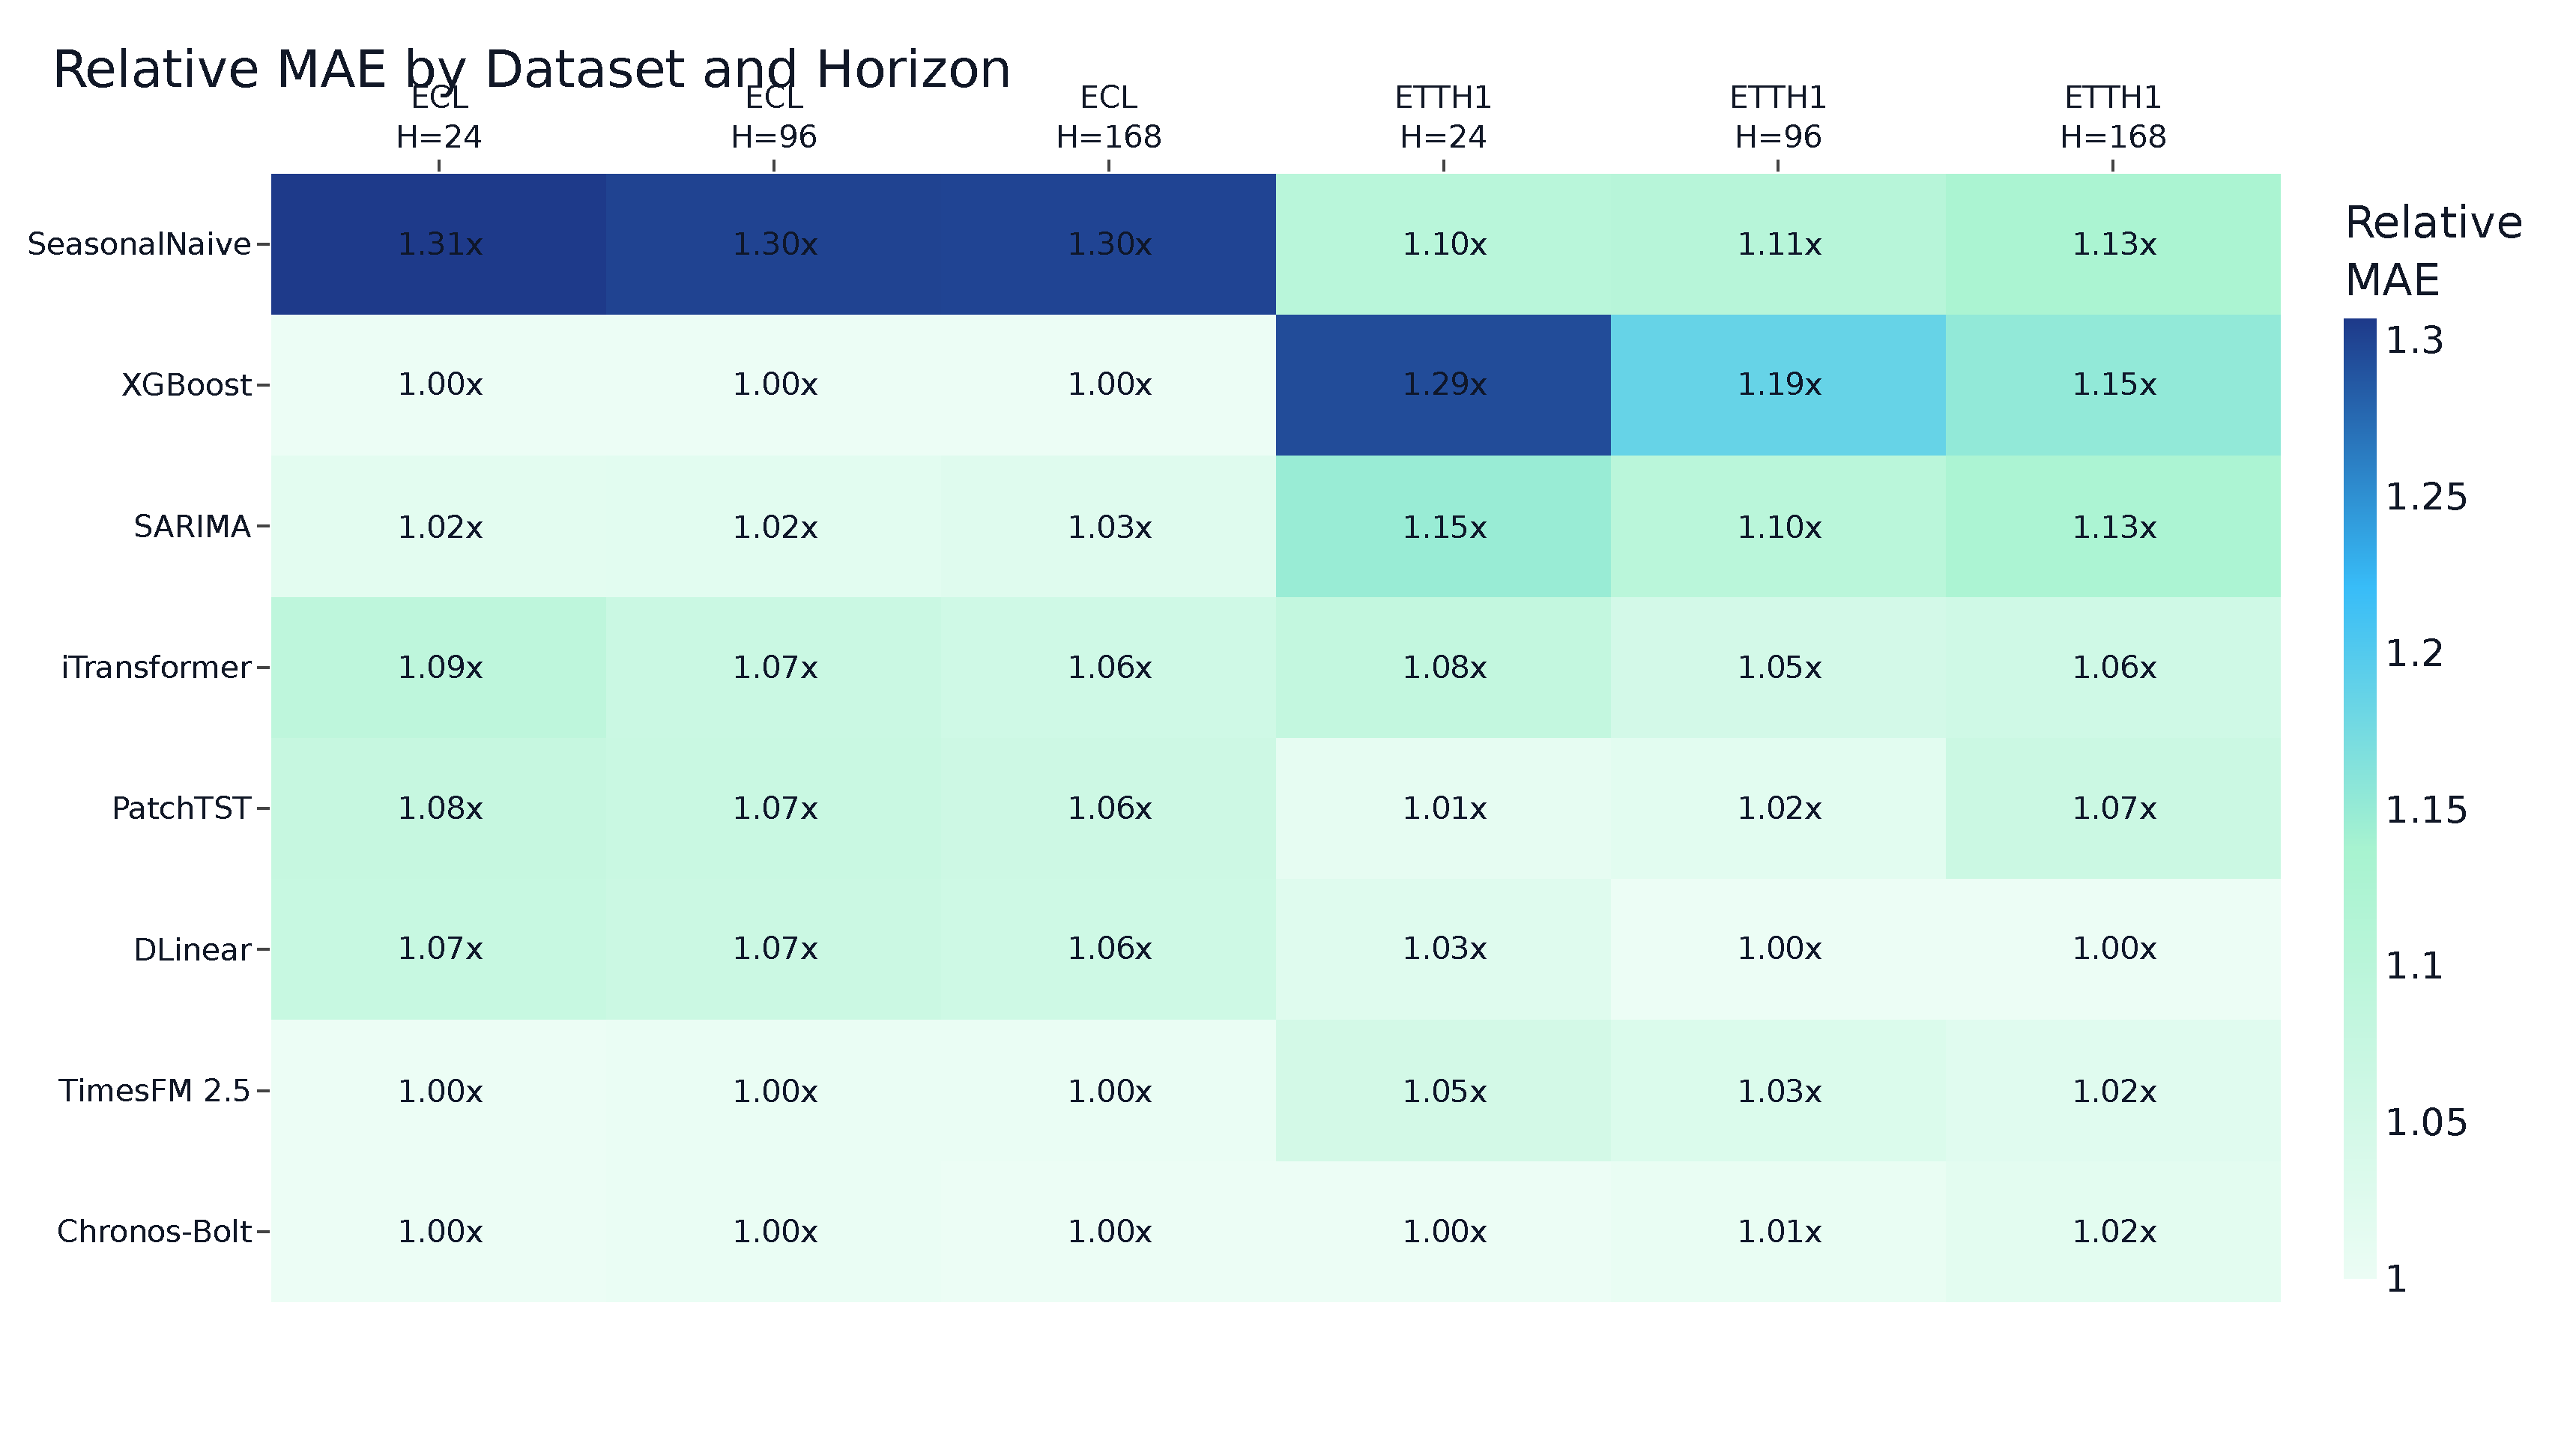
\includegraphics[width=\linewidth]{../figures/fig3_heatmap.pdf}
  \caption{Тепловая карта MAE по датасетам и горизонтам.}
  \label{fig:heatmap}
\end{figure}

\begin{figure}[t]
  \centering
  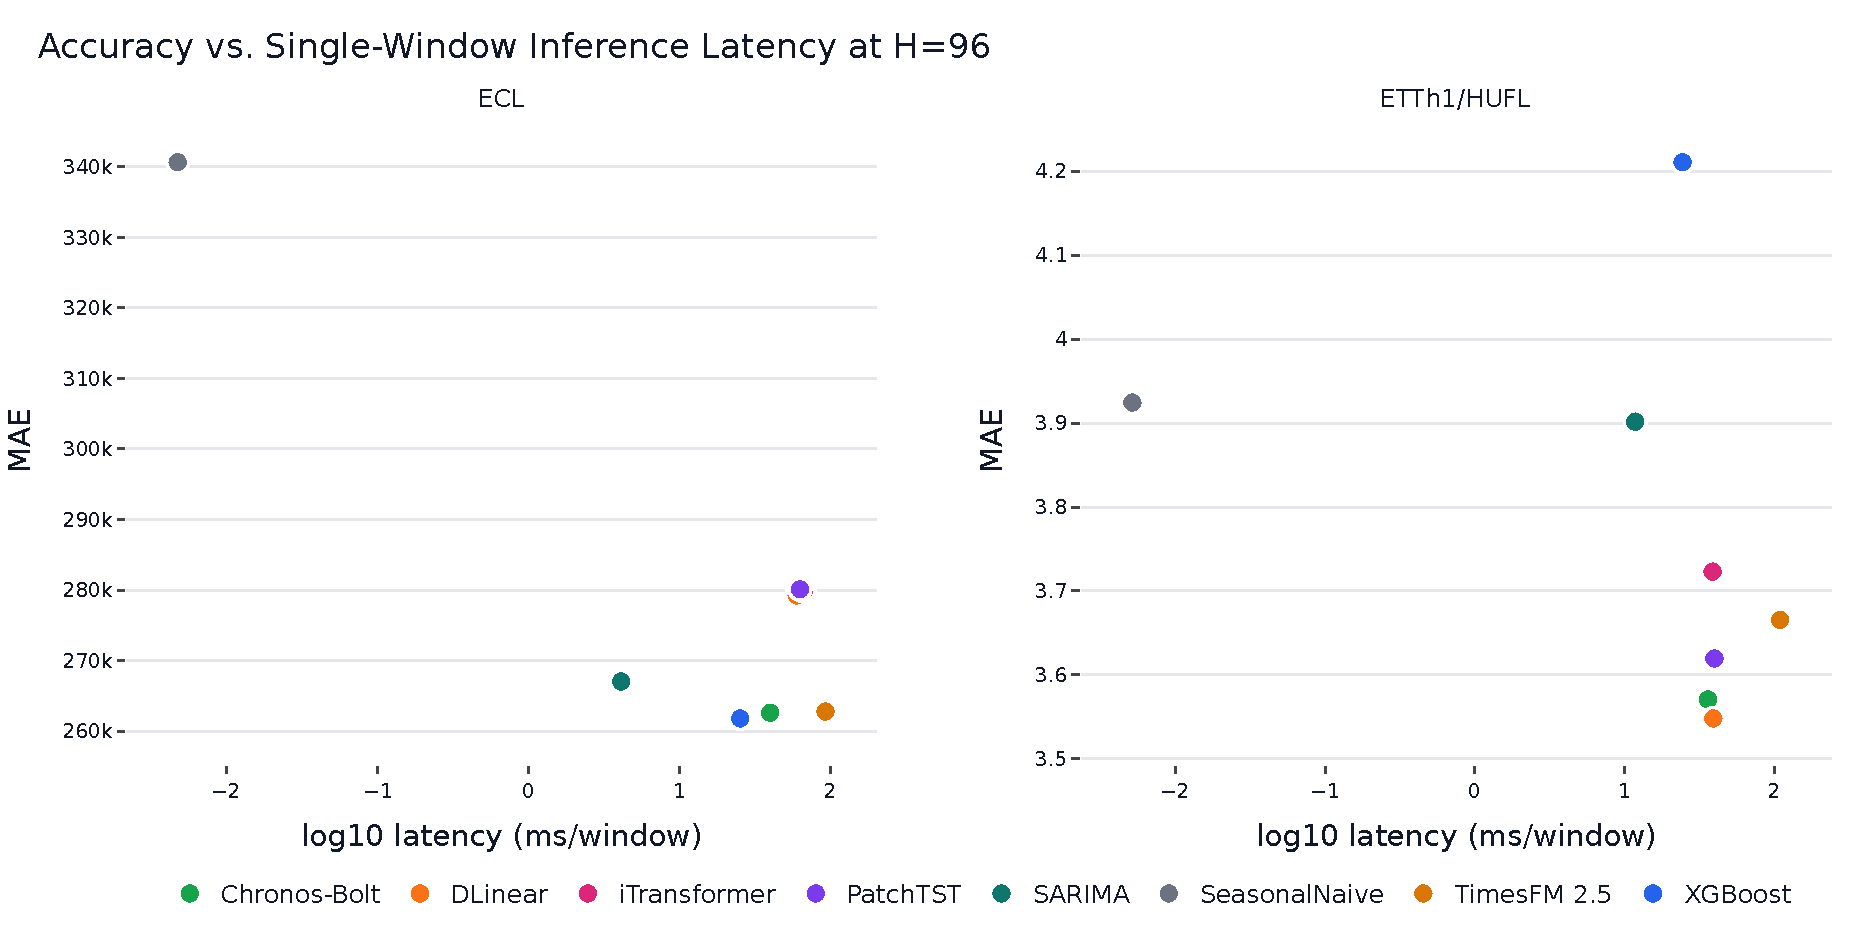
\includegraphics[width=\linewidth]{../figures/fig4_pareto.pdf}
  \caption{Accuracy--latency при H=96.}
  \label{fig:pareto}
\end{figure}

\begin{figure}[t]
  \centering
  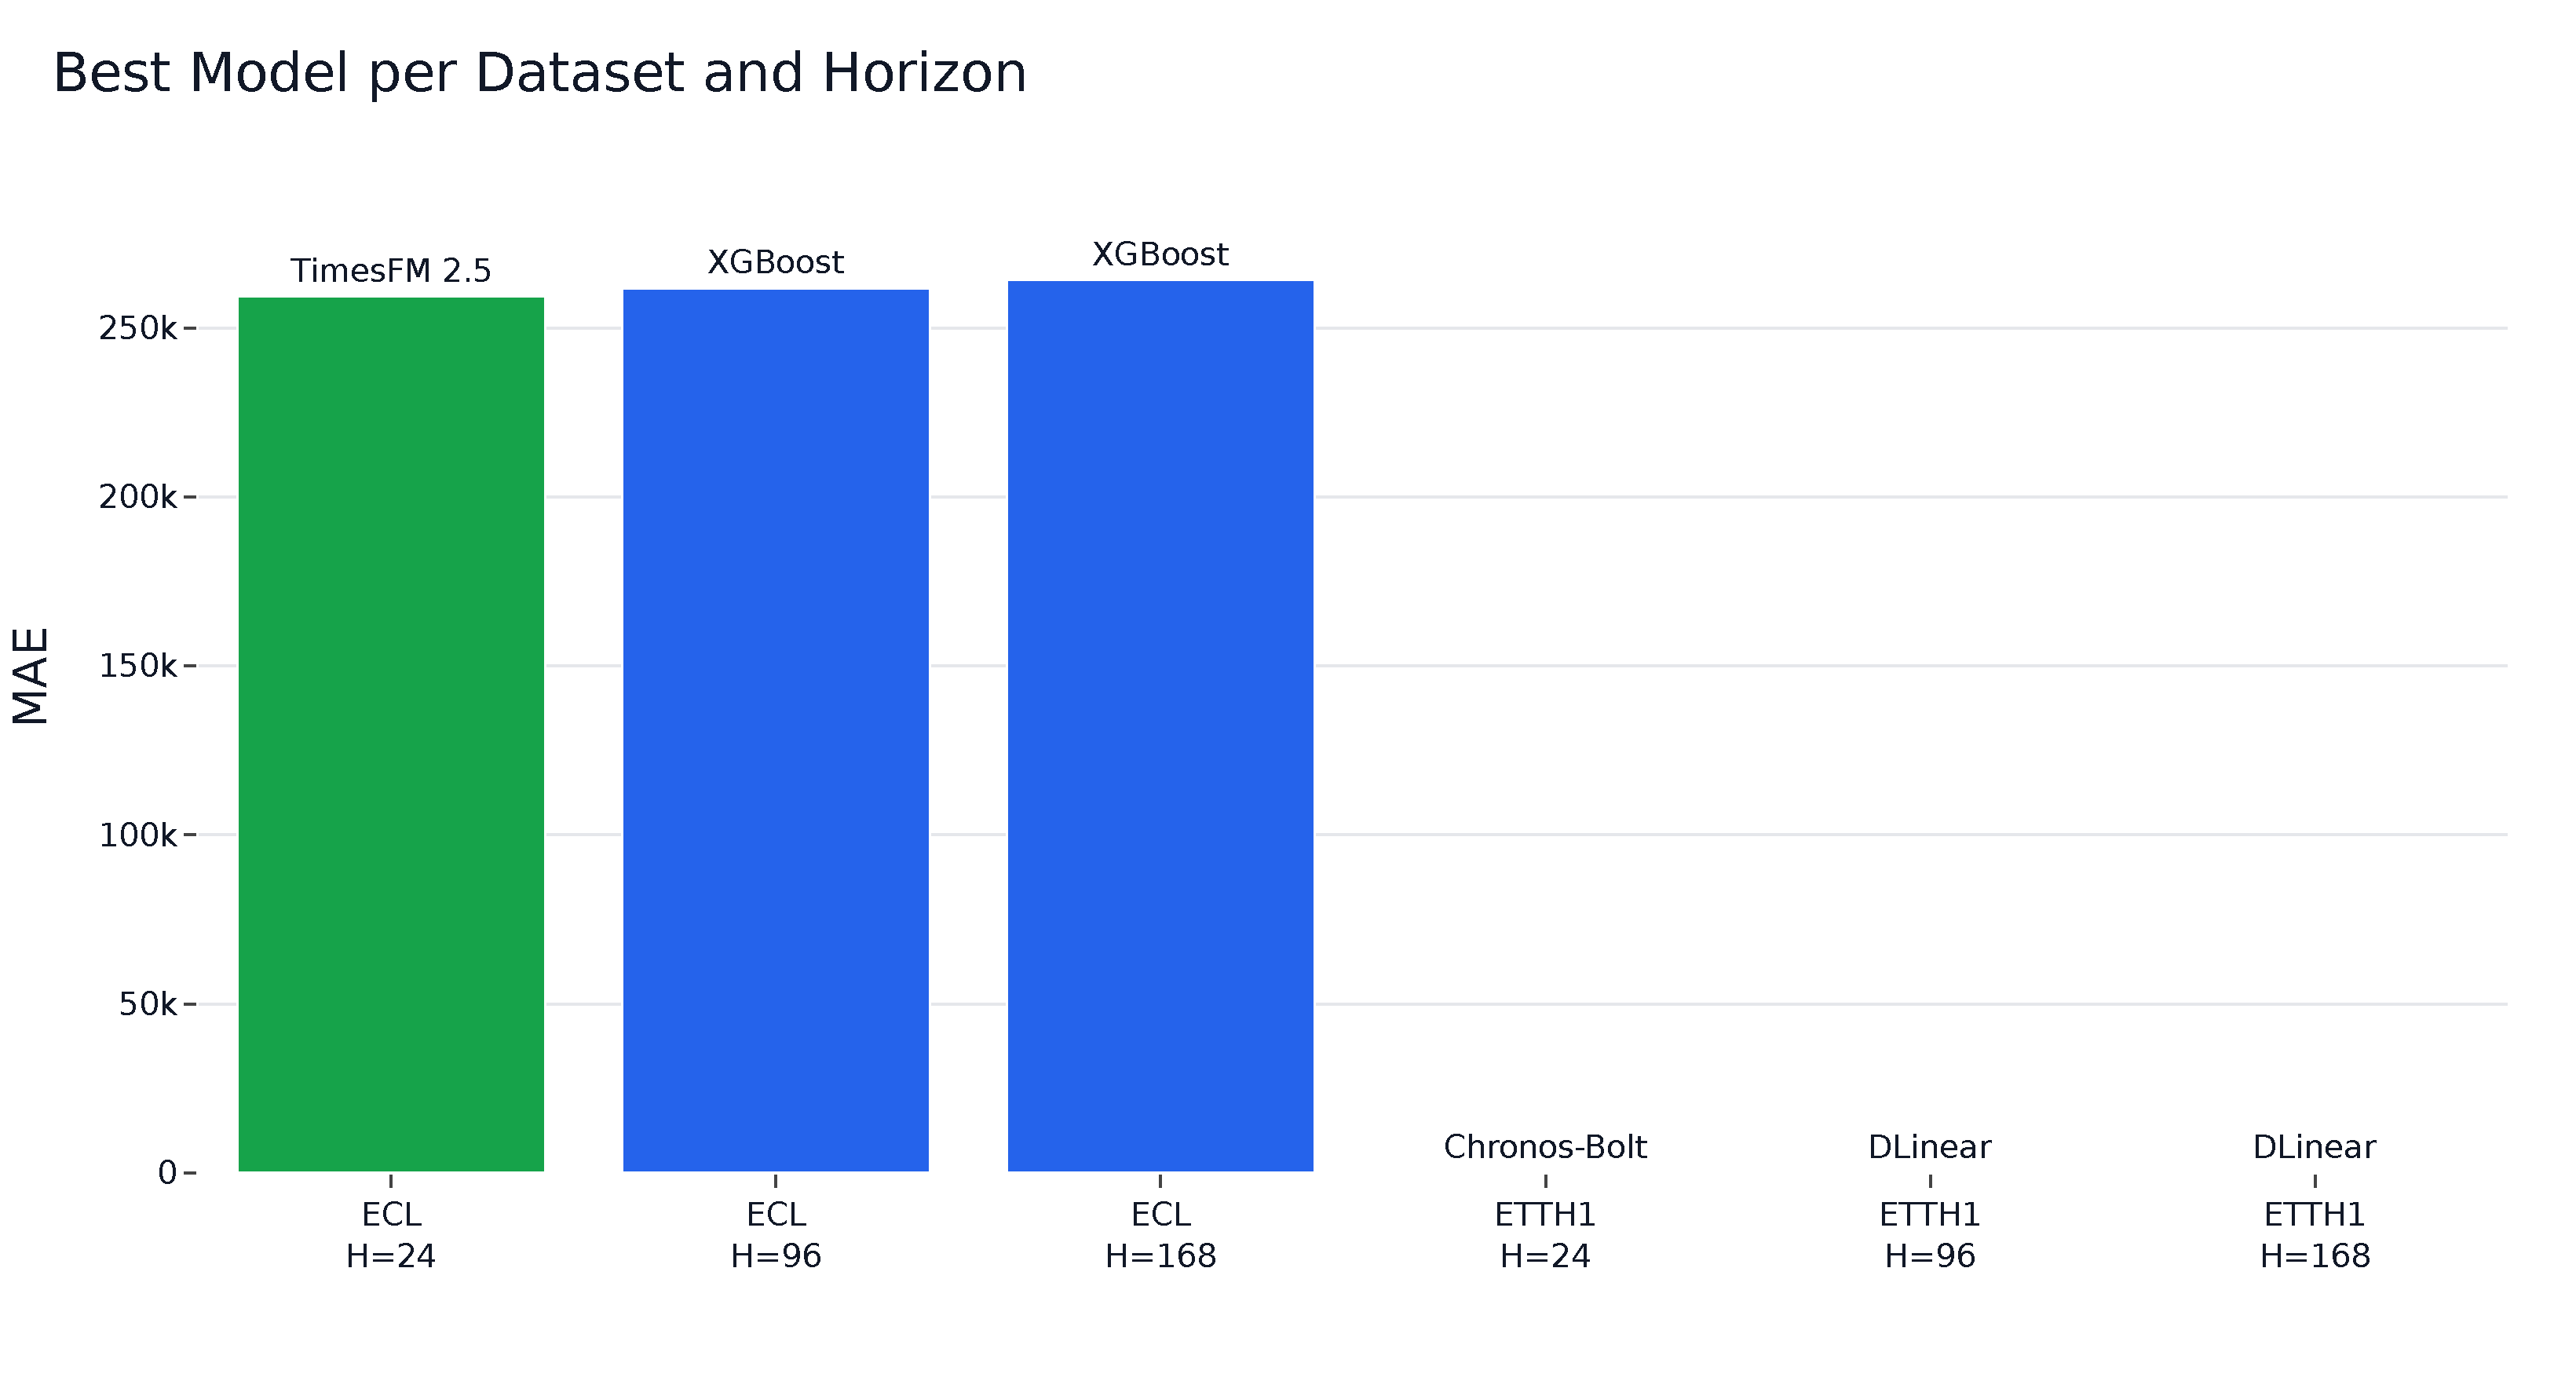
\includegraphics[width=\linewidth]{../figures/fig5_horizon.pdf}
  \caption{MAE по горизонтам.}
  \label{fig:horizon}
\end{figure}

\begin{figure}[t]
  \centering
  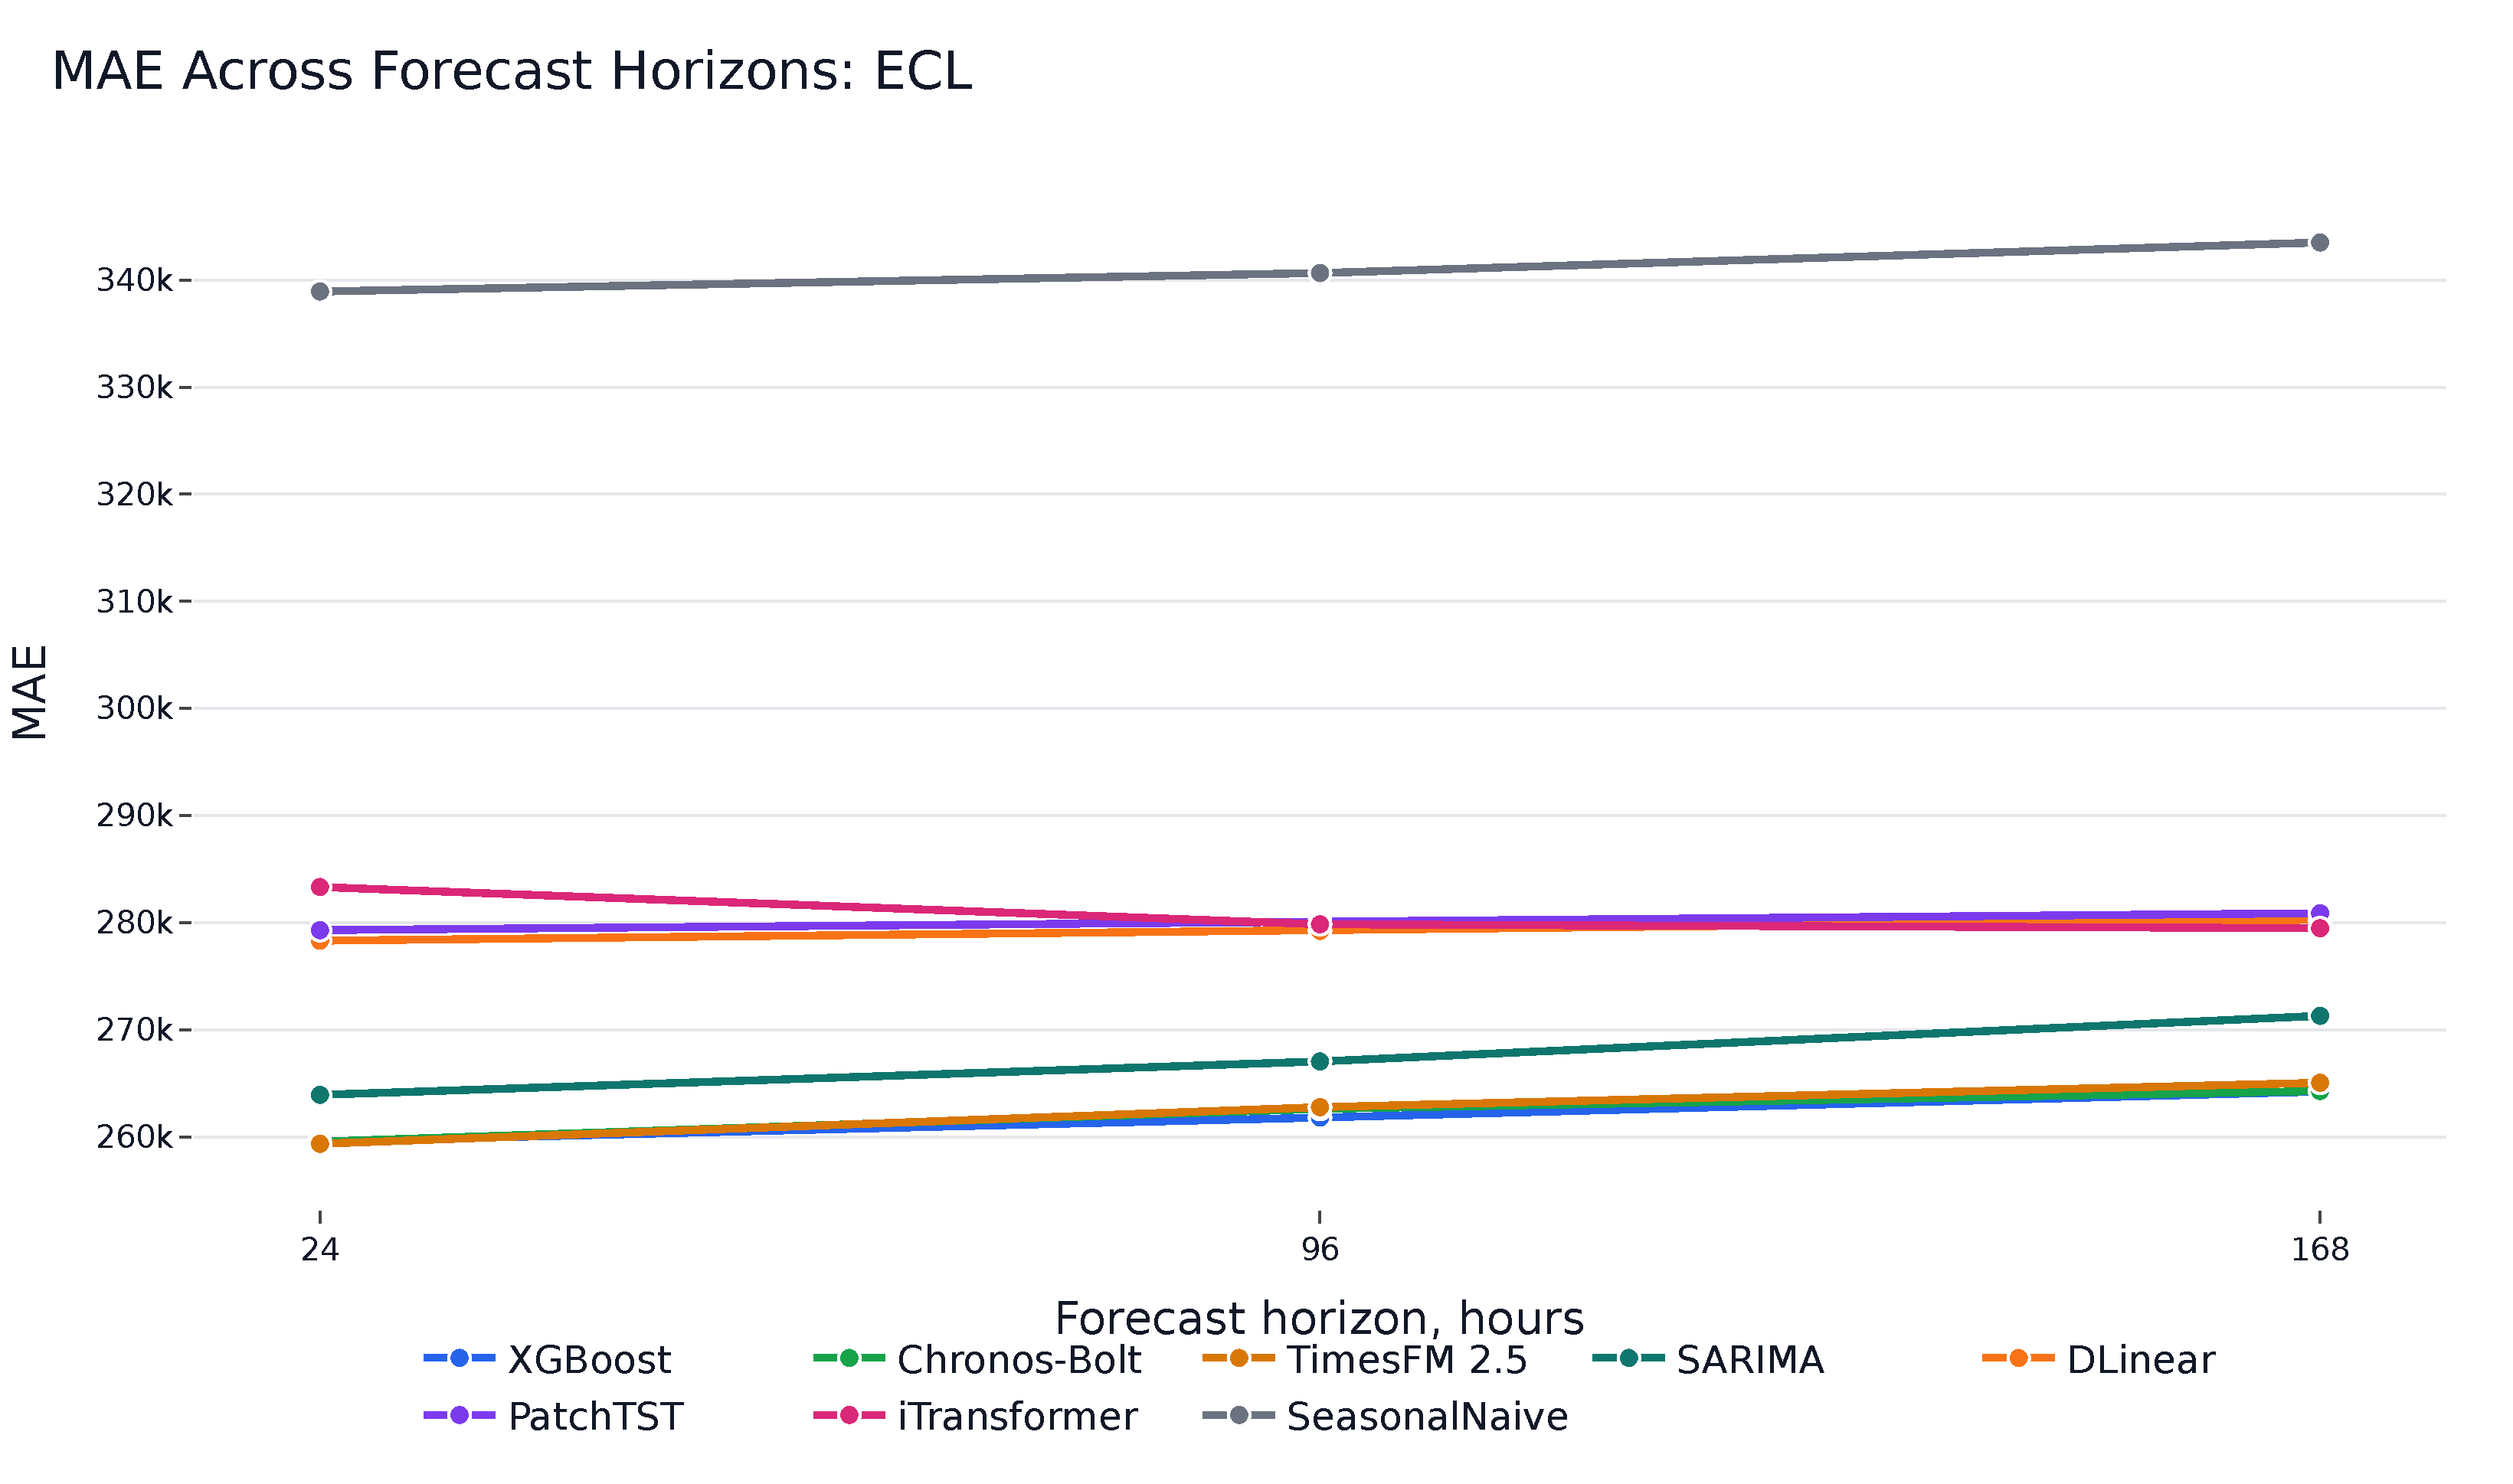
\includegraphics[width=\linewidth]{../figures/fig6_ecl_accuracy.pdf}
  \caption{MAE по горизонтам прогноза на ECL.}
  \label{fig:ecl_accuracy}
\end{figure}

\begin{figure}[t]
  \centering
  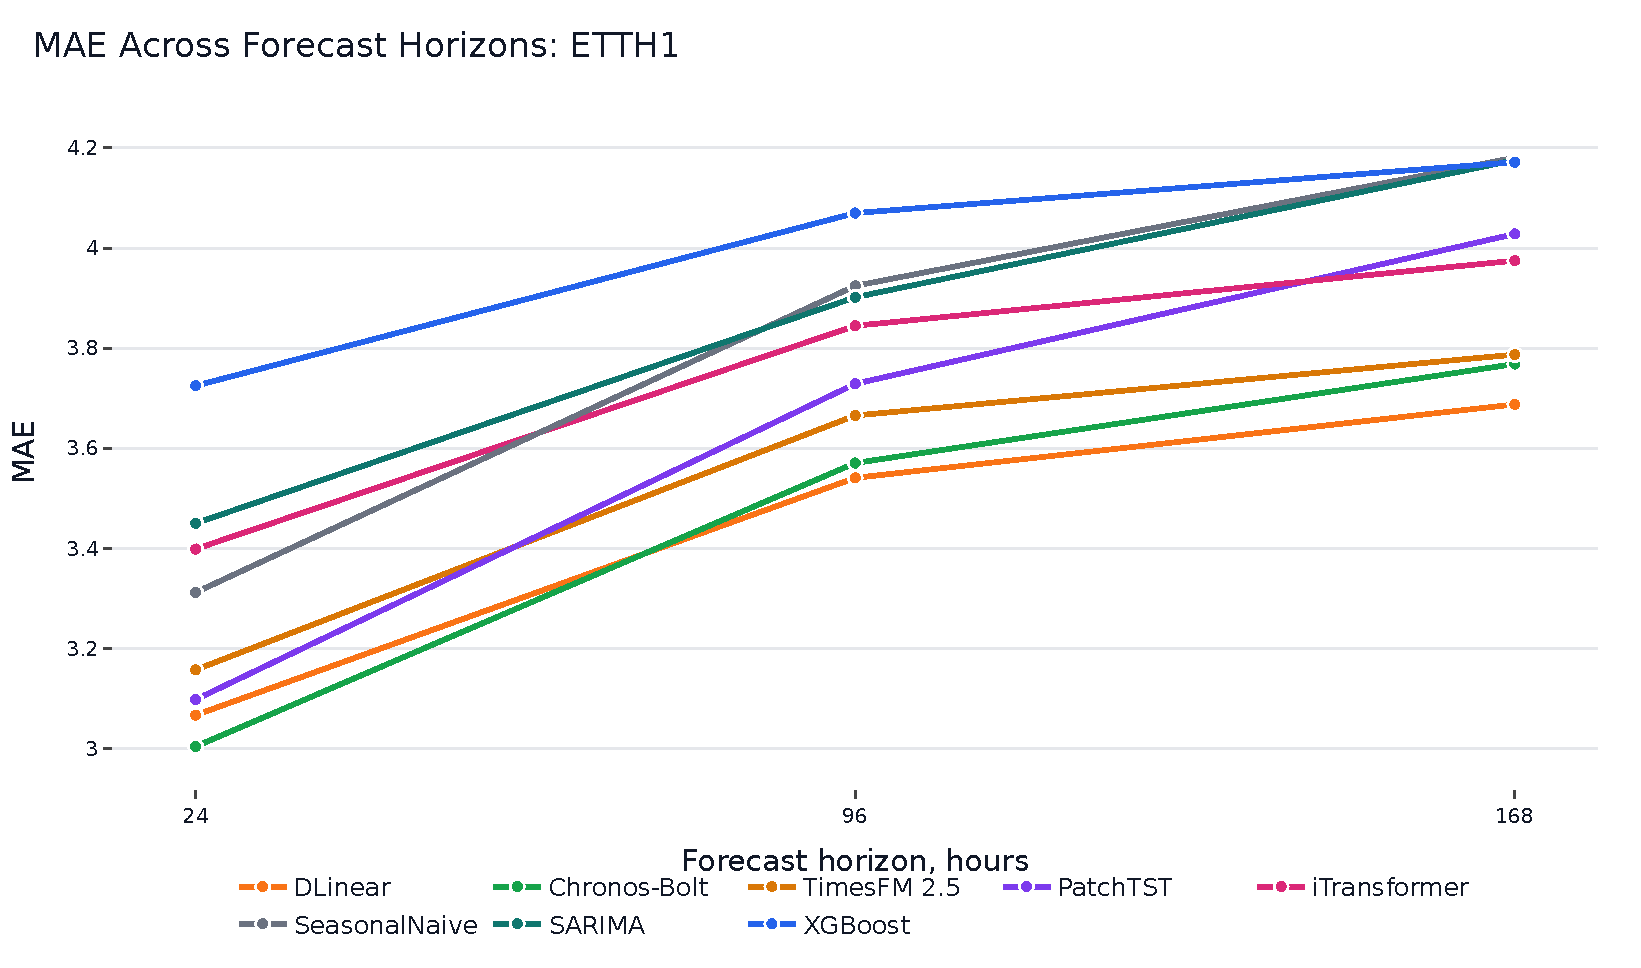
\includegraphics[width=\linewidth]{../figures/fig7_etth1_accuracy.pdf}
  \caption{MAE по горизонтам прогноза на ETTh1/HUFL.}
  \label{fig:etth1_accuracy}
\end{figure}

Accuracy--latency-визуализация (Рис.~\ref{fig:pareto}) и кривые MAE по датасетам (Рис.~\ref{fig:ecl_accuracy}, Рис.~\ref{fig:etth1_accuracy}) делают операционные режимы наглядными и согласуются с табличными ранжированиями.

\section{Обсуждение}
Результаты показывают, что выбор модели зависит от датасета. На агрегированной нагрузке ECL инженерия лагов в комбинации с XGBoost остаётся крайне сильным и недорогим решением, а грид-настроенный SARIMA --- следующая по точности модель, опережающая обучаемые нейросетевые архитектуры в этом сравнении. Фундаментальные модели привлекательны, когда отказ от обучения на целевом ряду имеет ценность: Chronos-Bolt близок к XGBoost на ECL и лучший на коротком горизонте ETTh1/HUFL. DLinear --- сильнейшая обучаемая нейросетевая модель в этом бенчмарке и доминирует на длинных горизонтах ETTh1/HUFL.

С точки зрения развёртывания модели занимают разные операционные режимы. XGBoost --- наиболее привлекательный выбор при допустимости стандартного supervised-пайплайна: точен на ECL, имеет малую single-window latency, не требует GPU. SARIMA --- конкурентный недорогой запасной вариант без обучаемых признаков и с миллисекундной инференсной задержкой. Chronos-Bolt полезен, когда обучение на целевом ряду нежелательно, например в сценариях cold-start промышленного мониторинга, быстрой прототипизации или когда данные нельзя объединять для обучения. TimesFM показывает сильную точечную точность на коротком горизонте ECL, но имеет существенно более высокую latency. DLinear --- хороший нейросетевой референс: простой, компактный и сильный на длинных горизонтах ETTh1/HUFL.

Результаты трансформеров стоит читать осторожно. PatchTST и iTransformer --- содержательные архитектуры, однако данный бенчмарк использует компактную одноцелевую конфигурацию и фиксированный бюджет обучения. Их относительная слабость здесь не означает общей непригодности трансформеров для прогноза нагрузки; она лишь показывает, что в условиях ограниченного и воспроизводимого протокола они не превосходят более простые методы автоматически. Производственное исследование должно включать более широкий перебор гиперпараметров, мультивариативные экзогенные входы и, возможно, датасет-специфичный тюнинг.

Основные ограничения связаны с риском контаминации фундаментальных моделей при претрейне на открытых бенчмарках, ограниченным перебором гиперпараметров, одноцелевым моделированием и отсутствием закрытых промышленных данных развёртывания. Скользящий AutoARIMA как базовая модель пробовался, но полный per-origin grid search оказался непомерно дорогим в этом протоколе; частичный запуск сохранён в логах репозитория, но исключён из основных таблиц сравнения. Грид-настроенный SARIMA в этой работе --- практическая замена: порядки выбираются на тренировочной выборке по AICc, и параметры повторно используются для окон прогноза, давая быстрый и чётко определённый ARIMA-базовый метод. Chronos-Bolt также выдаёт предупреждение о том, что длины прогноза свыше 64 находятся вне рекомендованного диапазона, поэтому результаты Chronos при H=96 и H=168 следует интерпретировать как практический стресс-тест, а не оптимальное использование модели.

Результаты фундаментальных моделей не следует чрезмерно интерпретировать как гарантированную zero-shot обобщающую способность на невиданных данных. ECL и ETT --- открытые бенчмарки, и они могут пересекаться с претрейнинговыми или оценочными корпусами, использовавшимися при разработке этих моделей. Корректное утверждение в этой работе уже: Chronos-Bolt и TimesFM запускались без обучения на целевом ряду в рамках данного репозитория. Это практически релевантно, но не равнозначно оценке на закрытом промышленном датасете.

\section{Заключение}
Построен и исполнен воспроизводимый пайплайн STLF-бенчмарка на ECL и ETTh1/HUFL. На ECL XGBoost, Chronos-Bolt и TimesFM статистически различимы, но операционно близки в пределах $0.4\%$, а грид-настроенный SARIMA --- ближайший преследователь; на ETTh1/HUFL Chronos-Bolt лидирует при H=24, PatchTST --- лучшая обучаемая модель на H=24, DLinear --- при H=96 и H=168. Эти выводы поддерживают прагматичную рекомендацию: сравнивайте сначала с сильными простыми базовыми методами, включая корректно настроенную модель ARIMA-семейства, используйте DLinear и PatchTST как нейросетевые референсы, а фундаментальные модели рассматривайте как ценный инструмент для cold-start, а не как универсально доминирующую замену supervised-прогнозированию.

\bibliographystyle{IEEEtran}
\bibliography{references}

\end{document}
